\documentclass[12pt,a4paper,oneside]{article}

\usepackage{polyglossia}
\usepackage{subfiles}
\usepackage{titlesec}
\usepackage{minted}
\usepackage{graphics}
\usepackage{adjustbox}
\usepackage{listings}
\usepackage{graphicx}
\usepackage{hyperref}

\usepackage{placeins}
\usepackage{flafter}

\usepackage{amsmath}
\usepackage{lipsum}
\usepackage{setspace}
\usepackage{systeme}
\usepackage{amsmath}
\usepackage{amssymb}

% \usepackage[demo]{graphicx}
% \usepackage{caption}
% \usepackage{subfigure}
\usepackage{subfig}

\usepackage{geometry}
\geometry{
    a4paper,
    total={170mm,257mm},
    left=20mm,
    top=20mm,
    left=22mm,
    right=20mm,
}

% Add bibliography
\usepackage[backend=biber, sorting=none, defernumbers=true, style=numeric]{biblatex}
\addbibresource{bibl.bib}

% Set line spacing
\renewcommand{\baselinestretch}{1.5}

% Disable spacing around list items
\usepackage{enumitem}
\setlist{nosep}

% Set font
\usepackage{fontspec}
\setmainfont{Times New Roman}

\setdefaultlanguage{latvian}
\SetLanguageKeys{latvian}{indentfirst=true}


\sloppy
\usepackage{fixlatvian}

\begin{document}

\begin{titlepage}
	\begin{center}
		\begin{figure}[ht]
			\centering
			
\includegraphics[width=60mm]{images/vea_logo.png}
		\end{figure}
		\large
		\textbf{Ventspils Augstskola \\Informācijas tehnoloģiju fakultāte}
		\vspace*{4cm}
		\\
		\textbf{Atskaite} \\
		\LARGE
		\textbf{Vienkāršas slimības izplatības simulācija}
		\vspace{0.5cm}
		\large
		\\
		mācību kursā \\,,Vizuālās programmēšanas valodas 2020"
	\end{center}

	\vspace{2cm}

	\begin{flushright}
		\normalsize
		\textbf{Izstrādāja:}\\
		Bakalaura studiju programmas ,,Datorzinātnes”\\
		3. kursa students\\
		Roberts Ivanovs \\
	\end{flushright}

	\vfill

	\begin{center}
		\Large
		Ventspils, 2020/2021
	\end{center}

\end{titlepage}



\clearpage
\tableofcontents
\clearpage

% Sections
\newpage
\section{Ievads}

% Problēma ko risina
\subsection{Problēma}

% TODO Add source of reference šitam paragrāfam
Viens no 2020 gada lielkājiem izaicinājumiem ir bijusi globālā \emph{COVID-19} pandēmija.
Šī slimība ir ļoti infekcioza, bet ne ļoti nāvējoša (vismaz ne jauniem cilvēkiem), tomēr
tā spēj ļoti ātri izsūkt visus spēkus no valsts medicīniskās sistēmas. Lai valdības spētu
pieņemt lēmumus par ierobežojumu ieviešanu, ļoti vērtīgi ir veikt dažādas simulācijas,
lai saprastu, kādā veidā slimība varētu progresēt un izplatīties sabiedrībā.

Šāda problēma noved pie projekta galvenā mērķa - \emph{veikt slimības izplatības modelēšanu}.

Mērķis tiks uzskatīts par sasniegtu, kad būs izpildīti sekojošie apakšuzdevumi:

\begin{enumerate}
    \item Vizuāla reprezentācija slimības procesa gaitai
    \item Iespēja pielietot slimības apturēšanas mehānismus
    \item Priekšnosacījumu konfigurēšana, lai ietekmētu simulācijas iznākumus
\end{enumerate}

% Tehniskie (personīgie) izaicinājumi
\subsection{Tehnoloģijas}

Ņemot vērā, ka kursadarba nosacījumos ir teikts, ka ir jaizmanto 3 dažādas kursa
laikā apskatītas tehnoloģijas, tad darba autors ir izvēlējies sekojošas tēmas:

\textbf{Blazor Server}\cite{blazor:info} - moderna WEB bāzēta tehnoloģija, kas darba autoram likās interesanta.
Interesei radīja, tas, ka darba autoram ir pieredze WEB sistēmu izstrādē un liela nepatika
pret JavaScript programmēšanas valodu, lai veidotu lietotāju saskarnes, uzskatot,
ka Blazor varētu būt labs alternatīvs nākotnes projektiem. Otrs apsvērtais
alternatīvs UI veidošanai, kas tika apskatīts studiju kursā - WPF - nestrādā uz
Linux, tāpēc to darba autors nevēlējās izmantot.

\textbf{Multithreading} - darba autoram iepriekš nav bijusi pieredze ar vairāku procesu
aplikāciju/sistēmu programmēšanu un uzskatīja, ka šis kursadarbs būs lielisks
veids kā apgūt zināšanas šajā jomā, iepazīstinātu sevi ar dažādiem konceptiem, kā
informācijas padošānu threadiem, objektu kopīgošanu un sistēmas paralelizēšanu.

\textbf{LINQ}\cite{linq:info} - darba autoram ir iepriekšēja pieredze citās programmēšanas
valodās ar dažādām funkcionalo valodu īpašībām, kā arī, ņemot vērā, ka šis
kursadarbs ir ļoti \emph{uz datiem vērsts}, tad LINQ ir loģiska izvēle šo datu
ērtai apstrādei un filtrēšanai ar C\# kodu.


\newpage
\section{Izstrāde}
\subsection{Projekta struktūra}
\subsection{Projekta struktūra}

Pirms sākot faktisko programmēšanu, darba autors veltīja laiku projekta
struktūras izplānošanai, lai veiksmīģiv arētu projetu realizet. Viens no šādiem
galvenajiem mērķiem bija atdalīt vizuālo lietotāju saskarni no pašas simulācijas.
C\# piedāvā diez gan labu risinājumu šādas projetkas struktūras attīstīšanai - izmantojot
\emph{namespaces} \cite{csharp:namespaces}. Tādējādi projekts tika strukturēts
divās galvenajās pakotnēs:

\begin{itemize}
    \item \emph{DiseaseCore} - atbildīgs par simulācijas veikšanu un programmiskā
        interfeisa piedāvāšanu, simulācijas veikšanai
    \item \emph{frontendserver} - atbildīgs par lietotāju saskarni
\end{itemize}

Šādu pieeju darba autors sākotnēji izvēlējās, jo nebija vēl pilnībā pārliecināts
par to, vai ar Blazor būs iespējams realizēt vēlamo projektu, tādēļ šadi atdalot
lietotāju saskarni no simulācijas koda, ar nosacījumu, ka simulācijas kods tiek
uzrakstīts pirms UI koda, varēs ērtāk \emph{pārlekt kuģus}, ja Blazor nebūs
iespējams izmatnot darbam un vajadžēs izmantto WPF. Lai gan darba izstrāde
izmantojot Blazor bija veiksmīga, tomēr šāda koda atdalīšana padarīja to ērtāk
menedžējamu, kad biaj nepieciešams veikt izmaiņas kodā, jo, paturot DiseaseCore
publisko interfeisu nemainīgu, bija ērti veikt izmaiņas pāšā simulācijas loģikā
pat pēc UI izstrādes, neradot papildus liekas koda kompilēšanas kļūdas.

\subsubsection*{Simulācijas koda struktūra}
% TODO Finish this


\subsubsection*{Lietotāja saskarnes koda struktūra}
% TODO Finish this


\subsection{Koda iekšējā struktūra}
\subsubsection{,,DiseaseCore" pakotne}
\subsubsection*{Multithreading}
Darba autors jau projekta plānošanas stadijā zināja, ka vēlēsies padziļināti
izpētīt un apgūt \emph{multithreaded} aplikācijas izstrādes principus, tāpēc jau pašā sākumā
centās saprast, kur projektā varētu veidot paralēlo darbību.

Šāda nepieciešamība noveda pie sekojošās koda arhitektūras, kuras vispārīgo
vizuālo reprezentāciju var apskatīt \ref{img:multithreaded-layout} attēlā: visa plakne, kur tiks
veikta simulācija, tiek sadalīta vienādos reģionos pa \(x\) asi (kods -- \emph{Region.cs} fails).
Katrā reģionā atrodas kaut kāda noteiktu sākotnējo entītiju (gan veselo, gan slimo) apakškopa,
tie tiek ievietoti savā reģionā no to attiecīgajām \(x\) ass koordinātām.

Katrs reģions tiek piešķirts noteiktai \emph{Task}\cite{csharp:task} instancei.
Tajā brīdī, kad noteiktais entītijs šķērso \(x\) \emph{Region} \(x\)ass robežu, tad tas tiek tiek
ievietots \emph{Out of bounds} buferī (kopīgs visām \emph{Region} instancēm), kuru
regulāri apstrādā cita \emph{Task} instance - katrs entītijs šajā \emph{Out of bounds} buferī tiek
izvērtēts pēc tā atrašanās vietas (pa \(x\) asi) un tiek novietos attiecīgā \emph{Region}
\emph{inbound} buferī, kuru brīvā brīdī noteiktā \emph{Region} pārvaldošais \emph{Task} pievienos
simulējamajiem entītijiem. Šo entītiju kārtošanas kodu var apskatīt
\ref{app:out-of-bounds-sorting} pielikumā.


\begin{figure}[H]
	\centering
	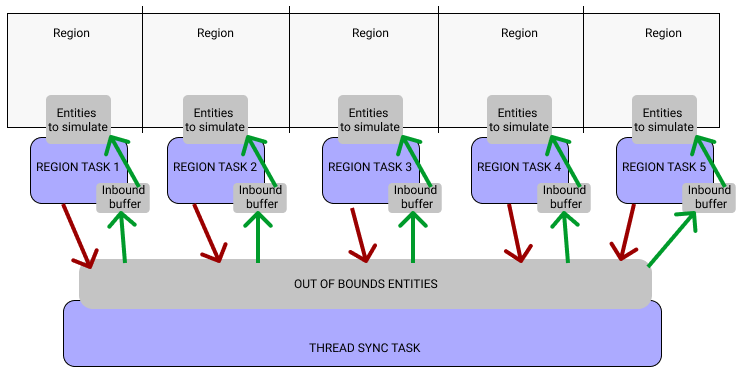
\includegraphics[scale=0.5]{images/multithreaded-layout.png}
	\caption{Reģionu sadalījums plaknei}
	\label{img:multithreaded-layout}
\end{figure}

Nepieciešamība izveidot \emph{inbound} buferi priekš \emph{Region} radās tādēļ, lai
nerastos situācija,
ka entītiju simulācijas brīdī (kur tiek veikta iterēšana pār entītijiem iekš \emph{Region}) pēkšņi
rastos kaut kādas modifikācijas no cita \emph{thread} -- \emph{data races}.

Izvēle dalīt visu simulācijas laukumu reģionos pa \(x\) asi (varēja būt arī \(y\)
ass, tikai ne abas asis reizē), bija tāpēc, lai ērti varētu to pielāgot dažādu
kodolu skaitam, ko var ērti realizet, ja plakne tiek dalīta tikai pa vienu asi.

Darba autors \textbf{neizmanto visus pieejamos procesora kodolus priekš \emph{Region} pārvaldības}, jo šādā gadījumā
procesors tiek pārslogots un tiek kavēta \emph{UI} atjaunošanās (par to
vēlāk tiks aprakstīts) -- tāpēc tiek izmantota tikai \(\frac{2}{3}\) no
pieejamajiem procesora kodoliem (vai sliktākajā gadījuma 1 kodols). Šī iemesla dēļ
\ref{img:multithreaded-layout} attēlā ir parādīti 5 reģioni/5 \emph{Tasks}/ \(\frac{2}{3}\) no 8 kodolu sistēmas.

Lai gan, ņemot vērā, ka \(1 Task\neq 1 Thread\), jo \emph{Taski} izpildās uz \emph{.NET Runtime}
pieejama \emph{threadpoola}\cite{csharp:tasks-not-threads}, tad reāli definēt vairāk
\emph{Tasks} arī ir iespējams -- \emph{runtime} definētie \emph{threadi} (mēdz saukt arī par
\emph{green threads}\cite{progr:green-threads}) izpildās
sistēmas \emph{userspace}\cite{sys:userspace}, nevis sistēmas \emph{kerneļa} līmenī, kas \emph{.NET Runtime}
atļauj pašam izlemt, kad darīt \emph{concurrent vai paralēlas}\cite{csharp:concurrent-parallel} darbības.
\emph{Tasku} pārvaldība
\emph{userspacā} ir daudz ātrāka nekā zemā līmeņa \emph{kerneļa threadu} veidošana.

Visi \emph{Task} dalītie resursi tiek ,,aizsargāti" ar \emph{Mutex}\cite{csharp:mutex}
instancēm, kas garantē to, ka informācija (aizsargātais mainīgais) netiks vienlaicīgi lasīts/rakstīts no
vairākiem citiem \emph{threadiem} vienlaicīgi -- datu integritāte tiek saglabāta. Izstrādes procesā
pareiza \emph{Mutex} implementācija radīja daudzas kļūdas -- \emph{data races} un \emph{deadlocks}.

% CHAPTER LINQ un Pipeline
\subsubsection*{Pipeline}

Lai sistēmā varētu nodrošināt funkciju modularitāti -- karantīna slimajiem,
definēti kopīgie saskarsmes punkti, \emph{zombie mode}, utt. -- bija nepieciešams
izplānot kādā veidā šo funkcionalitāti varētu ieslēgt un izslēgt koda izpildes
laikā. Darba autors izvēlējās funkciju kompozīcijas dizaina modeli --
\emph{Pipelines}\cite{progr:pipelines}. Pirms tiek izveidota galvenā simulācijas
instance \emph{World}(fails \emph{World.cs}), ir jāinicializē \emph{List} ar
\emph{Pipeline} (fails \emph{BasePipeline.cs}, skat. \ref{app:IPipeline} pielikumā)
interfeisa implementējošām instancēm. Interfeisa definīcija apskatāma sekojošajā kodā:

Objekts \emph{PipelineReturnData}, kuru atgriež \emph{pushThrough} funkcija ir
uzskatāms par \emph{type alias} \emph{Tuple<T, K>} mainīgajam:

{
\setstretch{1}
\begin{minted}{CSharp}
(List<EntityOnMap<SickEntity>>, List<EntityOnMap<HealthyEntity>>)
\end{minted}
}

, jo \emph{C\#} nepiedāvā valodas konstrukcij, kas atļautu definēt
\emph{type alias}. Šajā gadījumā tas tika darīts ar jaunas klases palīdzību, lai kods būtu lasāmāks.

Tālāk ir jāveido klases, kas implementē šo \emph{Pipeline} interfeisu -- katrai sistēmas
nepieciešamajai darbībai jāveido sava klases ar interfeisa implementāciju. Kopā
tika izveidoti 8 dažādi \emph{pipeline} objekti:

\begin{enumerate}
    \item \textbf{AttractorPipeline} -- definē rutīnas entītijiem, vietas uz kuriem visi kopīgi dosies.
    \item \textbf{DeathPipeline} -- izņem entītiju no saraksta, ja tā dzīvības ir vienādas ar \(0\).
    \item \textbf{GeoLocationPipeline} -- pārvieto entītiju kartē, aprēķinot tā jauno
        atrašanās vietu, zinot entītija virzienu, ātrumu, esošo lokāciju un pagājušo
        laiku kopš iepriekšējā \emph{pipeline} izsaukuma.
    \item \textbf{InfectionPipeline} -- pārbauda kuri veselie entītiji ir blakus slimajam
        entītijam un konvertē tos uz jauniem slimniekiem.
    \item \textbf{QuarantinePipeline} -- visus slimos entītijus novieto noteikta plaknes
        stūrī, lai izslimotu savu slimību.
    \item \textbf{RecoveryPipeline} -- ja slimais entītijs ir atveseļojies, tad konvertē to uz veselo entītiju.
    \item \textbf{TickingPipeline} -- iedarbina entītija ,,iekšējo" pulksteni (pārrēķina jaunu kustības virzienu, veselības stāvokli).
    \item \textbf{ZombieModePipeline} -- liek visiem slimajiem entītijiem virzīties pretī vistuvākajam veselajam entītijam.
    \item \textbf{AssertionPipeline} -- \emph{runtime} pārbaude vai visi entīiju tipi ir
        pareizi sadalīti (iepriekš tika izmantota dinamisku datu tipu
        kāstošana \emph{runtime} laikā, tāpēc šis pipeline bija
        noderīgs priekš kļūdu izķeršanas, bet šobrīd tā darbības jēga ir zudusi).
\end{enumerate}

Dažādie \emph{Pipeline}, kur tiek veiktas starp-entītiju pārbaudes, notiek tikai
katra \emph{Region} iekšējās robežās -- tas ir efektīvi sistēmai, bet \emph{Region}
dalījums par \(x\) asi dažreiz mēdz ierobežot entītiju uzvedību.

Sistēmas izstrādes laikā ir jāpievērš uzmanība arī \emph{pipeline} secībai, jo katrs \emph{pipeline}
operē ar iepriekšējā pipeline modificētajiem datiem -- izmainot secību
(vai arī izslēdzot/ieslēdzot kādu \emph{pipeline}) var rasties atšķirīgi iznākumi.

Katrai sistēmas \emph{Region} instancei ir pieejams inicializētais \emph{List<Pipeline>}
objekts, tad ar \emph{LINQ} palīdzību \emph{Region} izpildes ciklā tā iekšējos entītijus
,,izlaiž" cauri \emph{pipeline} sarakstam (\emph{Region.cs} failā, skat. \ref{app:pipelien-linq} pielikumā):

Papildus uzsvars uz \emph{LINQ} izmantošanu šajā kursa darba atskaitē nebūs veikts,
jo tas tika izmantots pilnībā visās \emph{Pipeline} implementācijās, gandrīz vai
visās simulācijas funkcijas un pat \emph{UI} saskarnē. Tika izmantotas dažādas šis
funkcionālas paradigmas metodes vairākās vietās kodā -- \emph{Aggregate, Where, Select, Concat, Min, Max, u.c.}.


\subsubsection{,,frontendserver" pakotne}

% Blazor UI kontrolē pipelines un instanciēšanu

Lietotāju saskarne ir programmēta ar \emph{Blazor Server} ietvaru. Sākotnēji darba
autors vēlējas izmantot \emph{Blazor WebAssembly} \emph{dotnet template} versiju,
lai varētu visu projektu novietot kā \emph{SPA}\cite{progr:SPA} uz statiskā faila servera. Tomēr
pašreizējā \emph{Blazor} versija nepiedāvā vairāku procesu paralelizācijas iespējas
(tikai \emph{concurrent} iespējamību, izmantojot vienu \emph{threadu}, kas arī ir
izmantots priekš pārlūkprogrammas \emph{UI} zīmēšanas)\cite{csharp:blazor-no-multithreaded-support}. Lai gan
visi \emph{WEB} brosweri kopš 2020 gada vasaras atbalsta \emph{WebAssembly Threads}
priekšlikumu \cite{wasm:threads-proposal}, tomēr to ir nepieciešams atsevišķi
,,ieslēgt" caur pārlūkprogrammas iestatījumiem. Otrs veids kā iegūt paralelizāciju \emph{WEB}
lietojumprogrammas ir ar \emph{WebWorkers}, bet lai to paveiktu, ir nepieciešama
papildus \emph{JavaScript} ,,līme".

\emph{Blazor WebAssembly} neatbalsta nevienu variantu vairāku
sistēmas \emph{threadu} izveidei. Šī iemesla dēļ tika izmantots \emph{Blazor Server}
versija, kur visa \emph{UI} apstrāde (arī simulācijas palaišana) notiek \textbf{uz servera}. Šāda
pieeja gan nozīmē, to, ka reāli uz serveriem publiskai pieejai šo sistēmu novietot nav laba doma -- jo
vairāk cilvēki pieslēgsies un veiks simulācijas, jo lielāka slodze un sliktāk tā strādās.
Tomēr tā ir problēma ārpus šī kursa darba ietvariem.

% Canvas pakotne
Pati attēla zīmēšana tiek veikta uz \emph{HTML5 Canvas} elementa\cite{html5:canvas}.
Šis elements piedāvā \emph{JavaScript API}, lai zīmētu reāla laika grafikas, attēlus, animācijas.
Tiek piedāvāti dažādi \emph{API} paveidi kā zīmēt lietas -- ,,2d", ,,webgl", ,,webgl2",
,,bitmaprenderer" \cite{html5:canvas-contexts}. Tomēr šie ir \emph{JavaScript API}, lai
no \emph{C\#} tos izsauktu, ir nepieciešams izveidot \emph{wrapper} funkcijas šim \emph{JS API},
nodrošinot starp-valodu komunikāciju. Darba autoram izdevās atrast jau izveidotu \emph{Blazor} bibliotēku,
kas nodrošina šo \emph{JavaScript API wrapper} priekš  \emph{HTML5 Canvas} -- \emph{BlazorExtensions.Canvas}
(\url{https://github.com/BlazorExtensions/Canvas}).
Darba autors jau iepriekš bija darbojies ar WebGL, kas nodrošinātu ātru un efektīvu
zīmējuma veidošanu un atjaunināšanu, tomēr šī \emph{BlazorExtensions.Canvas} bibliotēkas
dokumentācijā aprakstītais WebGL piemērs nestrādāja -- tāpēc darba izstrādē tika
izmantots ,,2d" \emph{context API}.

% Data polling
Inicializējot un uzstartējot simulāciju (skat. \ref{app:init-simulation} pielikumā), tā darbojas atsevišķā
sistēmas \emph{threadā} no \emph{UI} saskarnes -- no lietotāju saskarnes puses nav
viens konkrēts moments, kad
varētu iegūt visas nepieciešamās vērtības par esošajiem entītijiem sistēmā. Risinājums
ir izmantot tādu kā \emph{data polling}\cite{progr:data-polling} pieeju. pats Blazor koda \emph{polling}
pieeja ir apskatāma \ref{app:polling} pielikumā, bet simulācijas atbildi uz šo
vaicājumu var apskatīt \ref{app:polling-world} pielikumā. Koda sekvences
diagrammu priekš izveidotās \ref{app:polling-world} pielikuma metodes ir iespējams
aplūkot \ref{img:squance-diagram-get-status}
attēlā, bet pielikumā. Katrā
datu pieprasījuma reizē ir nepieciešams nepauzēt (iekšējais mainīgais, kas raksturo esošo stāvokli) visas \emph{Region} instances,
lai nenotiktu \emph{data races}, nepieciešams nepauzēt pašu \emph{World} instanci (lai
\emph{OutOfBounds} sinhronizācija nenotiktos datu nolases brīdī), tad nepieciešams apkopot
datus no visām datu krātuvēm, atpauzēt visas instances, atgriezt datus lietotāju saskarnei.

\begin{figure}[H]
	\centering
	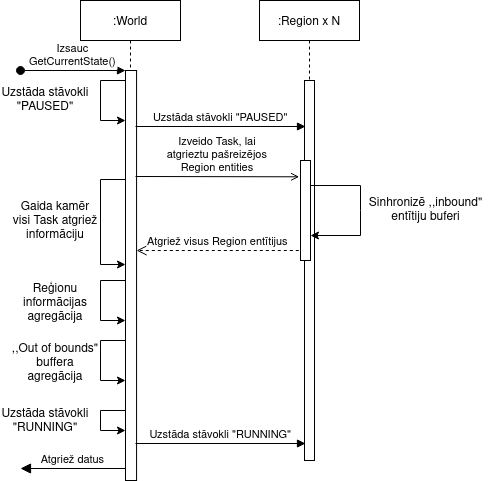
\includegraphics[scale=0.7]{images/DiseaseCore-GetData.png}
	\caption{Simulācijas datu stāvokļa vaicājuma izpilde}
	\label{img:squance-diagram-get-status}
\end{figure}

Tālāk šie iegūtie dati \emph{Blazor} pusē tiek papildus sadalīti: metadati tiek nodoti
\emph{Statistics} komponentei, kas aprēķina katra \emph{Region} ātrdarbību, bet
reāli dati par entītiju stāvokļiem tiek nodota \emph{Canvas} komponentei, kur
entītiji tiek sašķiroti un katrs uzzīmēts uz \emph{HTML canvas} ar \emph{BlazorExtensions.Canvas} bibliotēkas palīdzību.



\newpage
\section{Rezultāts}

% 2 sadaļas, footeris, main content

Izstrādāto galaprojektu ir iespējams uzstartēt ar \emph{shell} skrptu projekta
pamatdirektorijā \texttt{./start.sh}.
Projektu uzstartējot, apmeklējot ar interneta pārlūkprogrammu saiti
\url{https://127.0.0.1:5001/}, atvērsies lapa, kāda attēlota \ref{img:whole-ui} attēlā.

\begin{figure}[H]
	\centering
	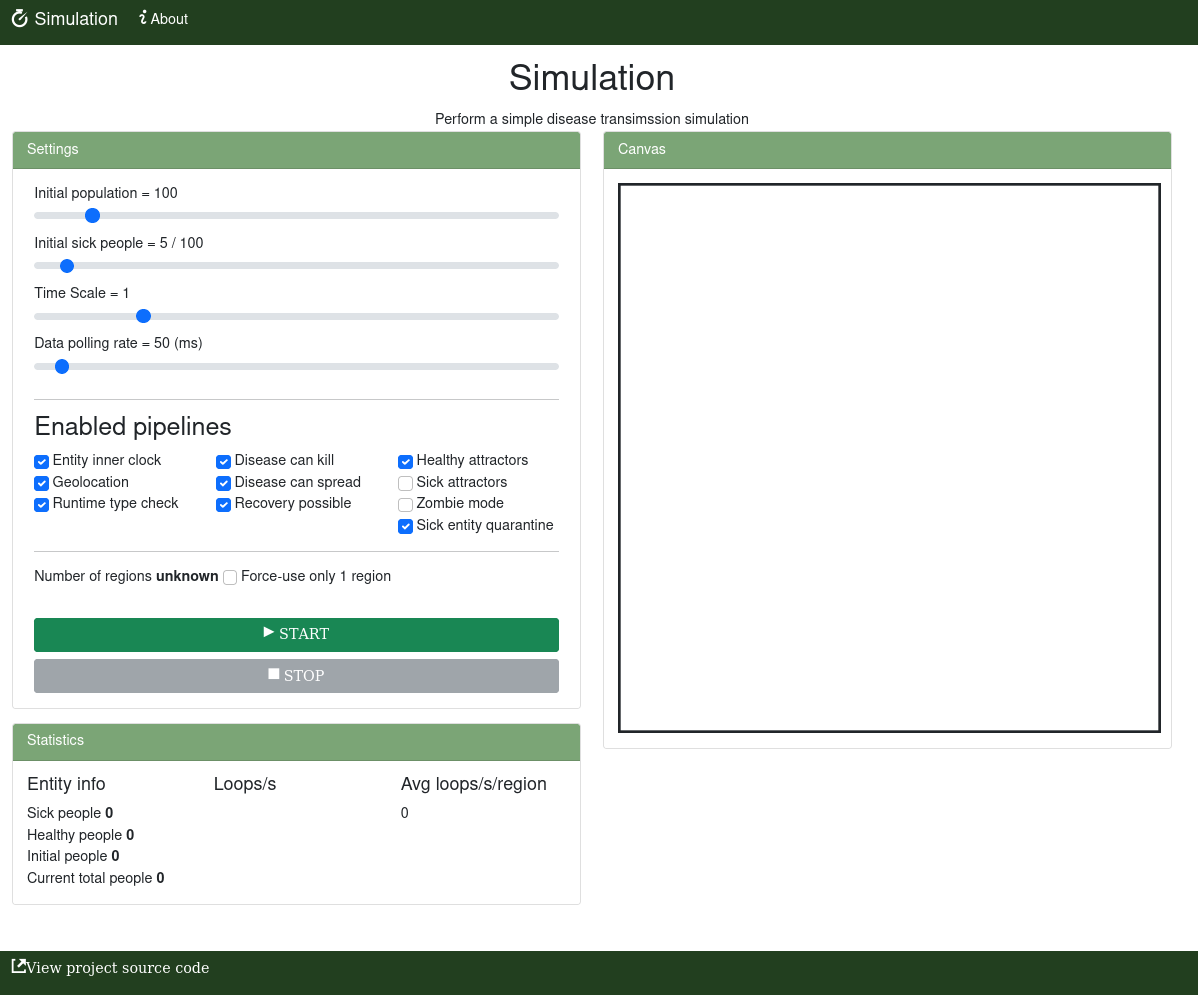
\includegraphics[scale=0.4]{images/ui-whole-page.png}
	\caption{Lietotāju saskarnes sākuma skats}
	\label{img:whole-ui}
\end{figure}

Lietotāju saskarne sastāv no divām lapām - pašas simulācijas (\ref{img:whole-ui}
att.) un ,,About" sadaļas (nav attēlots atskaitē).

% Settings panelis
\subsection{Iestatījumu panelis}

,,Settings" panelis ir galvenā vieta saskarnē, kur ir iespējams veikt sekojošās darbības:

\begin{itemize}
    \item \emph{Pipeline} ieslēgšanu/izslēgšanu,
    \item populācijas skaita maiņu,
    \item slimo entītiju skaita maiņu,
    \item datu pieprasīšanas intervāla (\emph{polling rate}) maiņu,
    \item iespēja piespiedus kārtā izmantot tikai vienu \emph{Region} instanci
    \item Uzsākt/apstādināt simulāciju
\end{itemize}

% Canvas
\subsection{Kartes komponente}

\emph{Canvas} elements attēlo simulācijā esošos entītijus lietotājam. Ņemot vērā, ka
simulācijas plaknes izmēri nesakrīt ar pikseļu dimensijām lietotāju saskarnes
\emph{canvas} elementa izmēriem, tad katrs punkts arī tiek normalizēts jaunajās
(lietotājam redzamajās) dimensijās. Zināmas problēmas gan rodas gadījumos, kur
ir liels entītiju skaits -- \emph{canvas 2d context} nespēj pietiekami ātri
uzzīmēt lielo elementu skaitu, rodas vizuāli artefakti. \emph{Canvas} elementus
ar dažādiem simulāciajs stāvokļiem dažādās stadijās var apskatīt \ref{img:canvas-show-off} attēlā.
Slimo entītiju krāsa mainās atkarībā no viņu veselības stāvokļa -- jo gaišāks, jo sliktāka veselība.

\begin{figure}[H]%
    \centering
    \subfloat
        [\centering Karantīna tiek ievērota (\emph{Healthy attractors} ieslēgts)]
        {{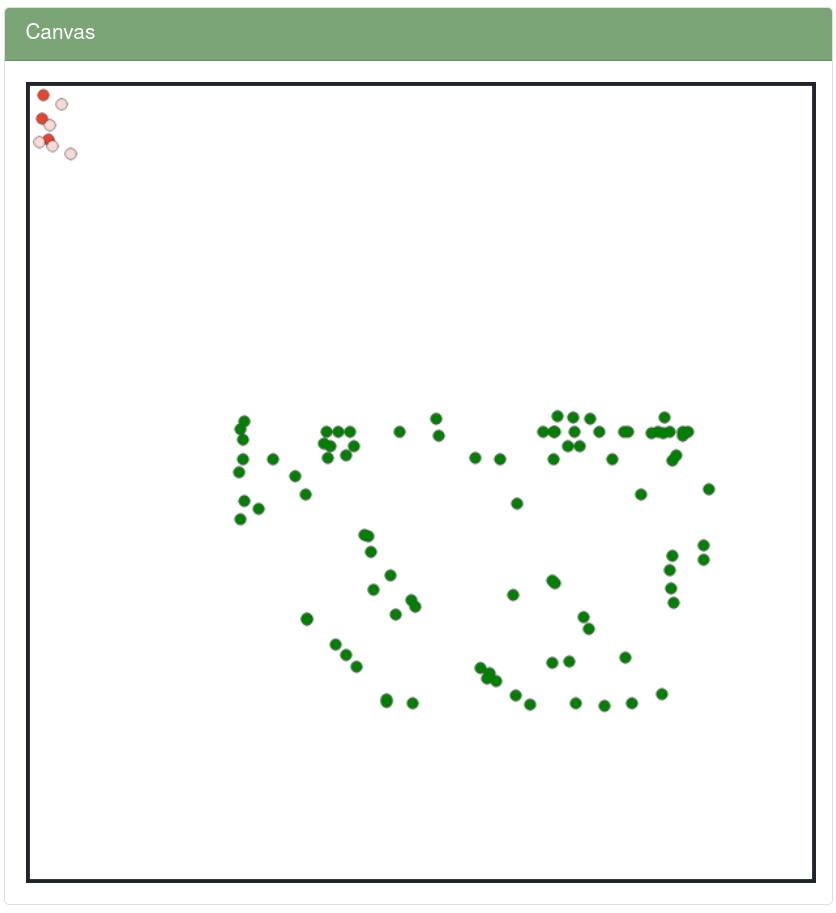
\includegraphics[width=.3\linewidth]{images/quarantine.png} }}%
    \qquad
    \subfloat
        [\centering Slimība izplatās, ja karantīna netiek ievērota]
        {{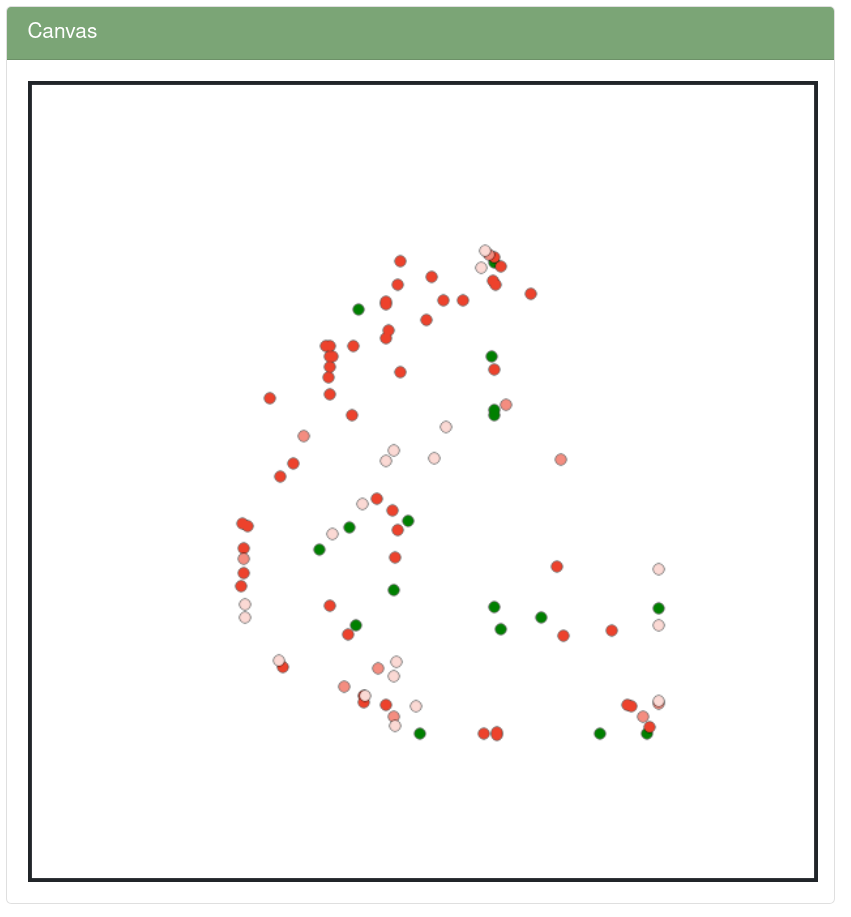
\includegraphics[width=.3\linewidth]{images/sickness-spreads.png} }}%
    \subfloat
        [\centering Atraktori ir izslēgti, ieslēgts \emph{Zombie mode}]
        {{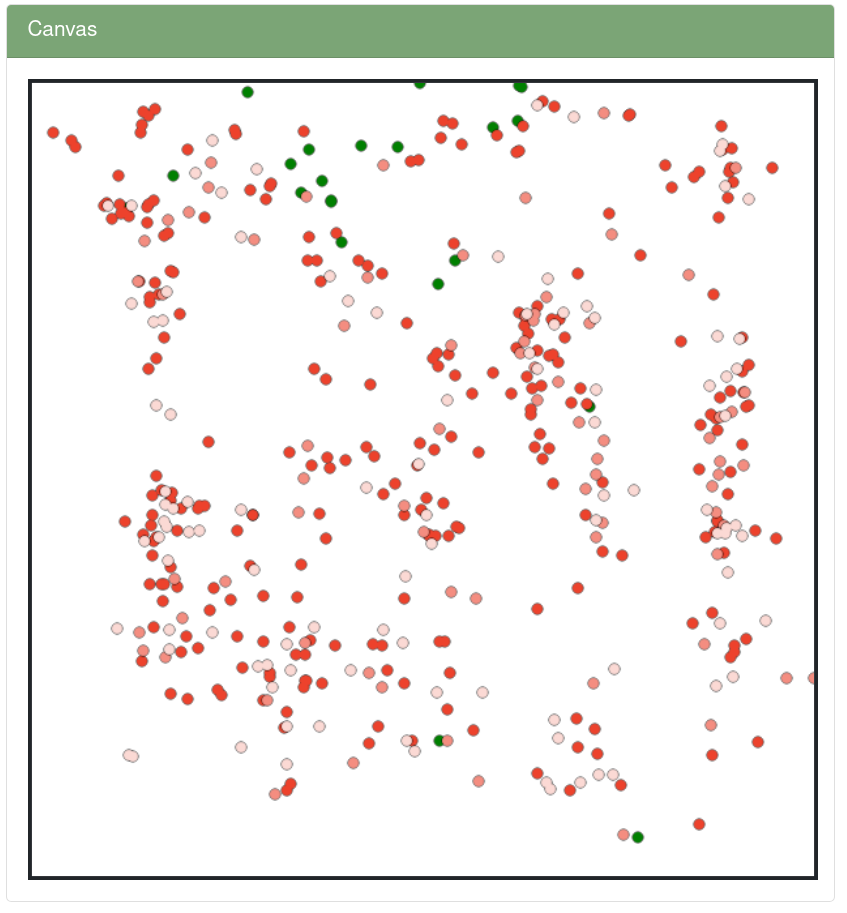
\includegraphics[width=.3\linewidth]{images/zombiemode-1.png} }}%
    \qquad
    \subfloat
    [\centering Ilgtermiņā turot ieslēgtu \emph{Zombie mode}, var redzet \emph{Region} sadalījumu]
        {{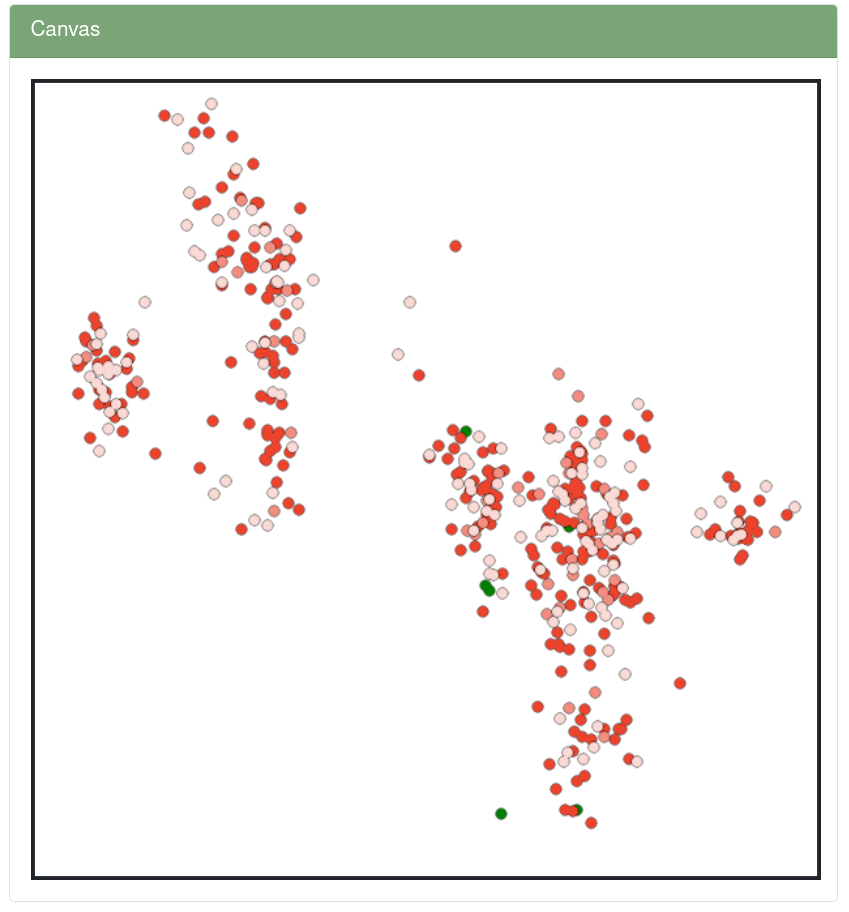
\includegraphics[width=.5\linewidth]{images/zombiemode-2.png} }}%
    \caption{Dažādu simulāciajs stāvokļu viuzalizācija}%
    \label{img:canvas-show-off}%
\end{figure}

% Statistics
\subsection{Statistikas komponente}

Tā kā \emph{canvas} vizualizācija der tikai kā uzskates materiāls, \emph{Statistics}
sadļa atļauj apskatīt to, kas notiek sistēmā ,,caur skaitļiem" (skat. \ref{img:statistics} att.).
Šī sadaļa ir sadalīta 3 kolonnās -- entītiju vispārīgā statistika, katra reģiona
noslodze (tiek mērīta ar iterācijām sekundē, kur 1 iterācija ir visu reģiona entītiju
izlaišana caur \emph{pipeline}, \emph{inbound} bufera pārbaude, entītiju ievietošana
\emph{out of bounds} buferī), bet 3. kolonna ir vidējāis aritmētiskais visu reģionu
noslodzei kopš simulācijas sākuma. Šie skaitļi atļauj ērti analizēt sistēmas
izmaiņas pie dažādiem iestatījumiem.

\begin{figure}[H]
	\centering
	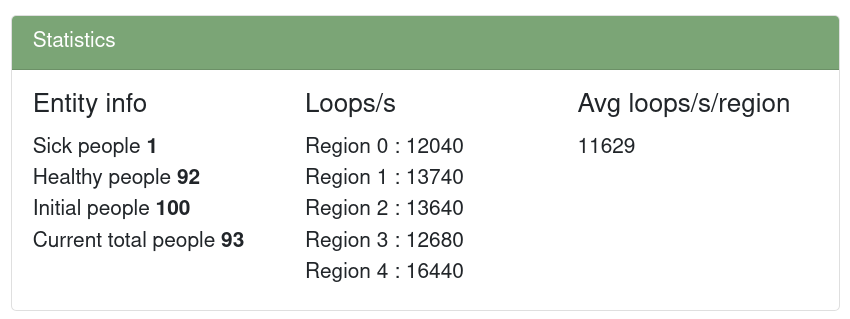
\includegraphics[scale=0.5]{images/statistics.png}
	\caption{Statistikas sadaļa}
	\label{img:statistics}
\end{figure}

\subsection{Vairāku-kodolu stresa tests}
% Max entities, no deaths, no nothing 1REGION vs 5 REGIONS
Izmantojot šo informāciju, kas apskatāma \emph{Statistics} komponentē, var veikt
nelielus testus esošajai programmai. Sākotnējais entītiju skaits tika uzlikts uz
maksimālo, lai pēc iespējas vairāk noslogotu procesoru, tad tika palaista programma
uz \~ 20 sekundēm, tikai ievākta informācija no sistemas. Šāda procedūra tika
atkārtota, izmantojot 1 \emph{Region} un 5 \emph{Region} instances. Rezultātus
ir iespējams apskatīt \ref{img:test-single-vs-mutlicore} attēlā.


\begin{figure}[H]%
    \centering
    \subfloat
        [\centering Statistika ar 1 \emph{Region} instanci]
        {{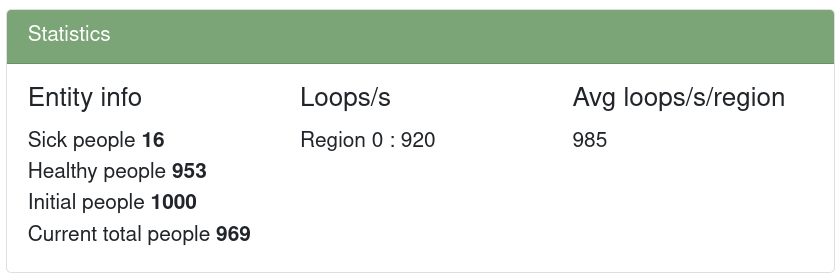
\includegraphics[width=.7\linewidth]{images/stress-statistics-single-sm.png} }}%
    \qquad
    \subfloat
        [\centering Statistika ar 5 \emph{Region} instancēm]
        {{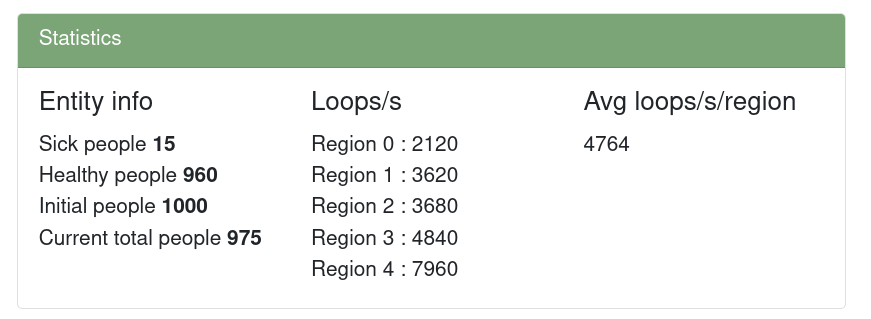
\includegraphics[width=.7\linewidth]{images/stress-stastiscs-multiple.png} }}%
    \caption{Sistēmas stresa tests}
    \label{img:test-single-vs-mutlicore}%
\end{figure}

Uz šo informāciju, ko attēlo šī komponente ir jāvērtē tikai kā ,,ieskats". Katru
reizi ģenerējot jaunu simulāciju, entītiji tiek uzģenerētei citās vietās, ar
dažādiem parametriem, atraktori tiek definēti dažādos daudzumos un dažādās vietās.
Protams, to visu ir iespējams statiski iekodēt kodā, lai tas nemainās, tomēr,
izstradājot sistēmu, mērķis nebija veikt padziļinātu analīzi par paralelizācijas
uzlabojumiem veiktspējā (ironiski, bet tiešī šī apakšadaļa to arī dara).


\newpage
\section{Secinājumi}
Darba autors uzskata, ka izstrādātā sistēma izpilda izvirzīto galveno mērķi
-- \emph{veikt slimības izplatības modelēšanu}. Kā arī
galvenie uzdevumi ir izpildīti -- ir nodrošināta vizuālā saskarne, iespēja
konfigurēt sistēmu un izpētīt slimības ierobežojošus mehānismus (karantīnas \emph{pipeline}).

Tomēr, darbu izstrādāt nebija viegli un darba autoram ir vairākas atziņas, kuras
var veikt, gan par pašu projektu, gan \emph{C\#} kā valodu un \emph{.NET ekosistemu} un \emph{WebAssembly}.

\begin{itemize}
    \item Darba autora primārā koda rakstīšanas vide is Visual Studio Code, kas
    nodrošina \emph{OmniSharp C\#} valodas serveri priekš \emph{C\#} koda intellisense,
    bet \emph{Razor} koda
    failu apstrāde lika tam regulāri pēkšņi pārtraukt darbību. Diemžēl citas alternatīvas
    nebija. Visos pārējos failos \emph{OmniSharp} strādāja ideāli, tomēr laikam tieši šim projektam
    \emph{(Blazor/Razor) OmniSharp} ir nepieciešama papildus uzmanība pilnīgam atbalstam.

    \item Darba autors nevarēja atrast labu koda stila \emph{linteri}, kuru būtu iespējams
    palaist no komandrindas, kas pieturētos pie \emph{C\#} dokumentācijā aprakstītā labā koda stila\cite{csharp:code-conventions}.

    \item \emph{Blazor} vēl nav reālas produkcijai gatavs risinājums priekš \emph{WebAssembly}.
    Bibliotēku atbalsts priekš \emph{DOM manipulāciajs} un \emph{JS API} ir niecīgs, reti uzturētas.
    Piemēram, vienīgā \emph{Canvas JS wrapper} bibliotēkai -- \emph{BlazorExtensions.Canvas} --
    nestrādāja \emph{WebGL API} (varbūt tā ir darba autora paša vaina? Tomēr
    dokumentācijā nekas nebija padziļināti par to rakstīts). Mūsdienās citām programmēšanas valodām kā \emph{Rust}
    ir daudz labāki risinājumi, piedāvājot vairākas alternatīvas \emph{OSS}
    bibliotēkas priekš \emph{JS API},
    \emph{WebAssembly} atbalsts kompilatoram ir \emph{first class citizen}, iespēju
    ērti veikt \emph{client-side multithreaded} darbus. C\# ekosistēmai un it
    sevišķi \emph{Blazor} vēl ir kur tiekties.

    \item Tā kā \emph{HTML canvas} ir
    \emph{JavaScript API}, tad katrs funkcijas izsaukums veic \emph{WebAssembly/JavaScript callback}
    funkciju padošanu ar vērtību klonēšanu -- jo vairāk šādas komunikācijas, jo
    lielāks lieks \emph{overheads} rodas (Viens no iespējamajiem faktoriem kāpēc \emph{canvas refresh rate} ir tik zems).

    \item \emph{Canvas ,,2d"} nav pietiekami jaudīgs priekš daudzu elementu reālā laika
    zīmēšanas. \emph{WebGL} būtu bijis labāks risinājums. \emph{Canvas ,,2d"} API nespēj veikt
    ātru, regulāru, liela apjoma datu attēlu atjaunošanu bez vizuāliem artefaktiem.

    \item \emph{Multithreading} aplikācijā, kur ir tikai vizuāla \emph{WEB} saskarne, nav vajadzīgs.
    Šādu sistēmu darba autors nekad neieteiktu nevienam likt uz serveriem.
    Darba autors uzskata, ka vislabākais, lai šo aplikāciju tik tiešām arī kāds
    varētu izmantot, būtu nepieciešams pārstrukturēt to kā 1 \emph{Region} aplikāciju
    (bez \emph{multithreading}) uz \emph{Blazor WebAssembly}, zīmēšanu veikt ar
    \emph{WebGL}, lai zīmējuma atjaunošanās būtu ātrāka. Varbūt, ja nākotnē \emph{C\#}
    atbalstīs arī jaunākus \emph{WEB} standartus, tad integrācija ar
    \emph{WebWorkers} būtu iespējama, lai veiktu sistēmas paralelizāciju ar vairākiem
    \emph{threadiem} -- bet šobrīd tas vēl nav iespējams.

    \item Būtu vērtīgi izpētīt, vai visu \emph{UI} atjaunošanās procesu varētu veikt ar
    \emph{requestAnimationFrame}\cite{web:req-anim-frame}. Jo pašreiz visa \emph{Canvas}
    zīmēšana notiek uz galvenā \emph{UI threada}, šis varētu būt pirmais
    optimizācijas veids, bet tam ir nepieciešama papildus \emph{JavaScript} ,,līme".

    \item Darba autoram \emph{pipeline} konstrukcija likās ļoti elegants risinājums
    sistēmas modularitātes problēmai, it sevišķi izmantojot \emph{LINQ}, priekš īsāka un lasāmāka
    koda. Ja otrreiz būtu jātaisa šāda sistēma, tad šo koda dizaina elementu
    noteikti arī dublētu jaunajā sistēmā.

    \item \emph{Mutex} konstrukcija ir obligāti nepieciešama, lai taisītu aplikāciju
    bez \emph{data-races}, tomēr \emph{C\#} valoda ir konstruēta bez papildus kompilācijas
    drošības nosacījumiem un \emph{Mutex} izmantošana ir ,,programmētāja labākajās
    interesēs, bet ne obligāta", kas var rast daudzas dažādas kļūdas, ja kāds mainīgais
    nav pareizi aizsargāts. Mūsdienās modernākām valodām kā \emph{Rust} un \emph{Go}
    ir pateicīgākas konstrukcijas priekš paralelizācijas (tīri teorētiski runājot,
    \emph{Rust} konstrukcija, kur \emph{Mutex<T>} ir \emph{generic} tips, ietverot
    sevī aizsargājamo objektu, liekas daudz ērtāk lietojama, tomēr
    darba autors praktiski ar paralelizācijām nav vēl strādājis šajās valodās un
    pašreiz tā ir tikai spekulācija).
\end{itemize}

Darba autors uzskata, ka mūsdienās eksistē labāki alternatīvi šāda projekta
izstrādei teju vai visos iespējamajos scenārijos -- lietotāju saskarnei \emph{TypeScript}
ar \emph{React}, bet, ja vēlme ir izmantot \emph{WebAssembly}, tad Rust piedāvā (pēc paša autora pieredzes
ar to strādājot) plašākas bibliotēkas ar labāku dokumentāciju un piemēriem. Tā arī būs visticamāk šī
projekta nākotne -- mēģināt to implementēt ar citām valodām un rīkiem, lai veiktu objektīvākus
salīdzinājumus.

Esošais projekts der tikai kā \emph{proof of concept}, ka kaut ko šādu var izstrādāt
un tas \emph{strādās}, bet tas nav projekts, kuru varētu novietot uz produkcijas
serveriem publiskai piekļuvei.


\newpage
\printbibliography

\newpage
\appendix
\section{Pipeline interfeiss}
\label{app:IPipeline}

Fails \texttt{BasePipeline.cs}
{
\setstretch{1}
\begin{minted}{CSharp}
    public interface Pipeline
    {
        void updateTimeScale(float timeScale);
        PipelineReturnData pushThrough(
            List<EntityOnMap<SickEntity>> currentSick,
            List<EntityOnMap<HealthyEntity>> currentHealthy,
            ulong timeDeltaMs
        );
    }
\end{minted}
}

\section{Pipeline datu izfiltrēšana ar LINQ}
\label{app:pipelien-linq}
Fails \texttt{Region.cs}
{
\setstretch{1}
\begin{minted}{CSharp}
    /* Izrēķina laika starpību kopš iepriekšējās iterāciajs */
    var current = sw.ElapsedMilliseconds;
    var timeDeltaMS = (ulong)(current - previous);
    /* Iterē cauri visiem pipeliniem */
    var pipelineResult = pipelines.Aggregate(new PipelineReturnData
    {
        // Inicializē ar sākotnējām Region vērtībām
        newHealthy = populationHealthy,
        newSick = populationSick
    },
    (aggregate, pipeline) => pipeline.pushThrough(
        aggregate.newSick, aggregate.newHealthy, timeDeltaMS
        )
    );

    // Saglabā izmainītās vērtības
    populationSick = pipelineResult.newSick;
    populationHealthy = pipelineResult.newHealthy;
\end{minted}
}

\section{Simulācijas inicializācija no Blazor}
\label{app:init-simulation}
Fails \texttt{Simulation.razor}
{
\setstretch{1}
\begin{minted}{CSharp}
    // Funkcija tiek izsaukta uzspiežot uz UI pogas
    async void StartSimulation()
    {
        /* Construct the pipelines */
        var pipelines = new List<Pipeline>();
        if (tickingPipeline) //<-- `bool` flags avaialble as checkboxes in the UI
            pipelines.Add(new TickingPipeline());
        if (deathPipeline)
            pipelines.Add(new DeathPipeline());
        if (infectionPipeline)
            pipelines.Add(new InfectionPipeline());
        /// .... Šādi iziet cauri visiem pieejamajiem pipeline....

        /* Construct the World object */
        simulation = new World(
            (ushort)(InitialPopulation - InitialSickPeople),
            InitialSickPeople,
            TimeScale,
            singleCore,
            pipelines);
        simulation.Start();
        /// ... Papildus algoritmam nesvarīgas darbības ...
    }
\end{minted}
}


\section{Galvenā polling funkcija no Blazor koda}
\label{app:polling}
Fails \texttt{Simulation.razor}
{
\setstretch{1}
\begin{minted}{CSharp}

// Šī funkcija iegūst informāciju no simulācijas
async Task ReloadInformation()
{
    await Task.Run(async () =>
        {
        var sw = new Stopwatch();
        sw.Start();
        var before = 0L;
        while (!startButtonEnabled)
        {
            var now = sw.ElapsedMilliseconds;
            var rerender = now - before > renderCanvasAfterEveryMiliseconds;
            // Veic darbību tikai tad, ja nepieciešamais laika
            // diapozons ir sasniegts
            if (rerender)
            {
                before = now;
                var gameState = simulation.GetCurrentState();
                /* Adjust the timing to be `loops per second` */
                var loopsPerSecond = gameState.loopsDone
                    .Select(
                        x => x * 1000 / (ulong)renderCanvasAfterEveryMiliseconds
                    )
                    .ToArray();
                simulation.timeScale = TimeScale;
                // atjauno vizuālo informāciju UI komponentēs
                await _statistics.setNewData(
                    gameState.sickPeople,
                    gameState.healthyPeople,
                    loopsPerSecond);
                await EntityCanvas.DisplayItems(gameState.items);
            }
        }
    });
}
\end{minted}
}

\section{,,Out of bounds" Entītiju kārtošanas mehānisms }
\label{app:out-of-bounds-sorting}
Fails \texttt{World.cs}
{
    \setstretch{1}
    \begin{minted}{CSharp}
        // ...
        // Iterate over all `outOfBoundsPopulation` and
        // figure out where should each item be placed
        foreach (var item in outOfBoundsPopulationSick)
        {
            // Normalise the location
            item.location.Y = Math.Min(
                Math.Max(item.location.Y, 1),
                World.MaxCoords.Y - 1);
            item.location.X = Math.Min(
                Math.Max(item.location.X, 1),
                World.MaxCoords.X - 1);
            // Place each item in its appropriate placeholder data container
            int index = item.location.X / deltaX;
            index = Math.Min(Math.Max(index, 0), regionManagers.Length - 1);
            inboundSick[index].Add(item);
        }
        // NOTE: The same algorithm is used for healthy entities as well
        // ...
        outOfBoundsPopulationHealthy.Clear();
        outOfBoundsPopulationSick.Clear();
        // Place each item in its appropriate thread
        for (int i = 0; i < regionManagers.Length; ++i)
        {
            if (
                (inboundSick[i].Count() > 0 || inboundHealthy[i].Count() > 0)
                && regionManagers[i].inboundAccess.WaitOne()
            )
            {
                regionManagers[i].inboundSick.AddRange(inboundSick[i]);
                regionManagers[i].inboundHealthy.AddRange(inboundHealthy[i]);
                regionManagers[i].inboundAccess.ReleaseMutex();
            }
            else
            {
                // Try appending the inbound item later
                outOfBoundsPopulationSick.AddRange(inboundSick[i]);
                outOfBoundsPopulationHealthy.AddRange(inboundHealthy[i]);
            }
        }
        outOfBoundsLock.ReleaseMutex();
        // ...
    \end{minted}
}



\section{Galvenā polling funkcija no simulācijas koda}
\label{app:polling-world}
Fails \texttt{World.cs}
{
\setstretch{1}
\begin{minted}{CSharp}

// Šī funkcija iegūst informāciju no simulācijas
public GameState GetCurrentState()
{
    this.SimState = SimulationState.PAUSED;
    ulong[] loopsDone = new ulong[regionManagers.Length];
    List<EntityOnMap<HealthyEntity>>[] populationHealthy = new List<
        EntityOnMap<HealthyEntity>>[regionManagers.Length];
    List<EntityOnMap<SickEntity>>[] populationSick = new List<
        EntityOnMap<SickEntity>>[regionManagers.Length];
    pipelines.ForEach(x => x.updateTimeScale(timeScale));
    // Pause all simulations
    for (int i = 0; i < regionManagers.Length; ++i)
    {
        regionManagers[i].SimState = SimulationState.PAUSED;
    }

    // Asynchronously extract the current state from each running task
    // Because the Region Tasks are still in the middle of a aloop right now
    Task[] waitingData = new Task[regionManagers.Length];
    for (int i = 0; i < regionManagers.Length; ++i)
    {
        int procIndex = i;
        waitingData[procIndex] = new Task(() =>
        {
            var item = regionManagers[procIndex].getEntities();
            populationSick[procIndex] = item.Item1;
            populationHealthy[procIndex] = item.Item2;
            loopsDone[procIndex] = item.Item3;
        });
        waitingData[procIndex].Start();
    }
    Task.WaitAll(waitingData);

    // SyncTaskCode() Task may still be running, therefore we lock it out
    // compeltely.
    outOfBoundsLock.WaitOne();
    var populationHealthyList = populationHealthy
        .Aggregate(
            new List<EntityOnMap<HealthyEntity>>(),
            (current, next) =>
            {
                current.AddRange(next);
                return current;
            }
        )
        .Concat(outOfBoundsPopulationHealthy)
        .ToList();
    var populationSickList = populationSick
        .Aggregate(
            new List<EntityOnMap<SickEntity>>(),
            (current, next) =>
            {
                current.AddRange(next);
                return current;
            }
        )
        .Concat(outOfBoundsPopulationSick)
        .ToList();
    outOfBoundsLock.ReleaseMutex();

    // Resume all paused states
    this.SimState = SimulationState.RUNNING;
    for (int i = 0; i < regionManagers.Length; ++i)
    {
        regionManagers[i].SimState = SimulationState.RUNNING;
    }

    // Gather metadata
    var sickPeople = (ushort)populationSickList.Count();
    var healthyPeople = (ushort)populationHealthyList.Count();

    // Return the result
    return new GameState
    {
        loopsDone = loopsDone,
        items = (populationSickList, populationHealthyList),
        sickPeople = sickPeople,
        healthyPeople = healthyPeople,
    };
}
\end{minted}
}


\end{document}
